%!TEX root = ../report.tex

\chapter{Evaluation}

\section{Densenet}

In Densenet each layer connects to every layer in a feed-forward fashion. 
With the basic idea to enhance the feature propagation, each layer of Densenet blocks takes the feature-maps of the previous stages as input.  


\subsection{Siamese densenet structure}

Where the branches of the Siamese network are Densenet. 
% Commands to include a figure:
\begin{figure}[h]
\centering
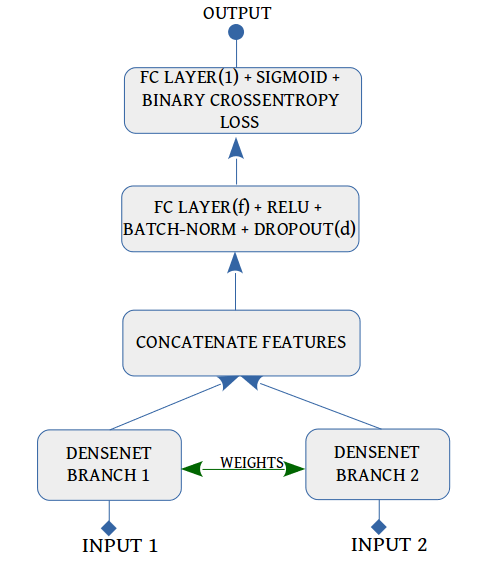
\includegraphics[width=0.5\textwidth]{images/densenet/siamese_densenet_structure.png}
\caption{\label{fig:dn_siamese}Siamese densenet structure.}
\end{figure}

\section{Hyperparameters}
Hyper-parameters are those parameters whose values are set before the training, unlike other parameters whose values are learned during the training. 
For example learning rate, batch size. \cite{wikihyper}
\subsection{Parameters of Densenet}
